\documentclass{report}

\usepackage{amssymb}
\usepackage{amsmath}
\usepackage{amsthm}
\usepackage{kpfonts}
\usepackage{tikz}
\usepackage{wrapfig}

\usetikzlibrary{matrix, arrows}

\DeclareMathOperator{\lcm}{lcm}
\DeclareMathOperator{\im}{im}

\title{Group Theory}
\author{Jacob Denson}
\date{\today}

\begin{document}

\maketitle

\chapter{Basic Definitions and Properties}

\section{What is a group?}

A group is a set of objects which can operate with each other. One can find them almost anywhere in mathematics, from number theory to geometric symmetry. The goal of this course is to learn and understand the properties that all groups have.

We begin with a definition of how objects operate with each other. A law of composition or assignment on a set $S$ is a function from $S \times S$ to $S$. If $a$ and $b$ are arguments to this function, the value mapped from $a$ and $b$ is denoted $a \circ b$, $ab$, $a + b$, and pretty much any other symbol you can think of. Given a positive integer $n$, we write $a^n$ for $a \circ a \circ \dots \circ a$ $n$ times.

An assignment is associative if for any three elements $a$, $b$, and $c$, $a(bc) = (ab)c$. All in all, this means that any brackets are redundant in an equation. Formally, there is a unique way of defining a sequence $[a_1 a_2 \dots a_n]$, such that for any $a$, $[a] = a$, for any $b$, $[ab] = a \circ b$, and for any integer $i$ from $2$ to $n$, $[a_1\ \dots\ a_n] = [a_1\ \dots\ a_{i-1}] \circ [a_i\ \dots\ a_n]$:
\begin{proof}
    We prove by induction that for any set of $n$ elements, $[a_1\ a_2\ \dots\ a_n]$ is uniquely determined. With only one element, the uniqueness is obvious, as is the case for two elements. Now suppose any product of $n-1$ elements is uniquely defined. Note by splitting up the sequence, we know the sequence is unique, so we need only find one that works. Define $[a_1\ a_2\ \dots\ a_n] = [a_1\ a_2\ \dots\ a_{n-1}] \circ a_n$. Let $i$ be an arbitrary integer from $2$ to $n-1$. The following calculation shows we can split up our sequence in that way.

    \begin{align*}
    [a_1\ a_2\ \dots\ a_n] &= [a_1\ a_2\ \dots\ a_{n-1}] \circ a_n\\
    &= ([a_1 \dots a_{i-1}] \circ [a_i \dots a_n]) \circ a_n\\
    &= \underbrace{[a_1 \dots a_{i-1}] \circ ([a_i \dots a_n] \circ a_n)}_\text{Associativity is used here}\\
    &= [a_1 \dots a_{i-1}] \circ [a_i \dots a_n]
    \end{align*}

    The transition from $1.2$ to $1.3$ is where the associative property of the assignment is required.
\end{proof}

An example of an associative operation on a set is, for any two element $a$ and $b$, $a \circ b = a$. Then $a \circ (b \circ c) = a \circ b = a$, and $(a \circ b) \circ c = a \circ c$. Thus the operation is associative.

Another property of an assignment is commutivity: that for any elements $a$ and $b$, $a \circ b = b \circ a$. Given associativity, a sequence is equal to any permutation of its elements. That is, if $a_1, a_2, \dots, a_n$ are a sequence of elements, and $\pi$ is a permutation of $1$ to $n$, then $a_1\circ a_2 \circ \dots \circ a_n = a_{\pi(1)} \circ a_{\pi(2)} \circ \dots \circ a_{\pi(n)}$.
\begin{proof}
    We prove by induction. This is obvious for one element. Suppose this is true of permutations of $n-1$ elements. Let $i$ be the integer such that $\pi(i) = n$. Then the following calculation shows we can move $a_i$ to the end of the sequence.

    \begin{align*}
    a_1 \circ a_2 \circ \dots a_i \dots \circ a_n &= (a_1 \circ a_2 \circ \dots a_i) \circ \dots \circ a_n\\
    &= \underbrace{a_{i+1} \circ \dots \circ (a_1 \circ a_2 \circ \dots a_i)}_\text{Commutivity is used here}
    \end{align*}

    Now renumber each element from $1$ to $n-1$. Then our original permutation is a permutation of $n-1$ elements when restricted to the first $n-1$ numbers, so we may by induction permute these remaining numbers to get the correct ordering required by the permutation $\pi$.
\end{proof}

Note that it is assumed that an operation is commutative if the symbol $+$ is used for the operation.

An identity of a set and assignment is an element $e$ that is idempotent, that is, that $a \circ e = e \circ a = a$ for any element $a$. There can only be one such $e$ for if we have another idempotent element $e'$, we have that $e = e' \circ e = e'$. If $\cdotp$ is used for the operation, we may write $e$ as $1$, and if $+$ is used, we may write it as $0$, even though the element is not always a number. If a set has an identity, we define, for any element $a$, $a^0 = e$.

Given a set with an identity $e$, we say an element $a$ is invertible if there is another element $b$ such that $a \circ b = b \circ a = e$. b is normally denoted $a^{-1}$, or if $+$ is used for the operation, $-a$.

Here are some common properties of inverses. We assume associativity, but not commutivity in our operation. Let $a$, $l$, and $r$ be arbitrary elements, and $e$ the identity:
\begin{itemize}
    \item If $la = e$ and $ar = e$, then $l = r$, and $a$ is invertible:
    \begin{proof} Then $l = le = lar = er = r$ \end{proof}
    \item $a^{-1}$ is unique:
    \begin{proof} The above property shows any two inverses are the same, behaving as $l$ and $r$ in the above proof. \end{proof}
\end{itemize}

A monoid is a set with an associative operation that contains a unit element (so the monoid is also non-empty). We say a monoid is commutative or abelian if its operation is commutative. Inverses are not required. The order of the monoid is the number of elements it contains.

Some examples of monoids are the following. You should be able to come up with infinitely more (One could probably write the ``Encyclop\ae dia of Monoids''):
\begin{itemize}
    \item The set of non-negative integers under addition
    \item The set of positive integers under multiplication.
\end{itemize}

The main topic of this class is the concept of a group: a monoid where every element has an inverse. We can use this to extend exponentiation. If $n < 0$, define $a^n = (a^{-1})^{-1}$.

We require inverses for a group, but we can weaken this claim only requiring left inverses. It turns out that if for every element in a monoid $G$ has a right inverse, every element also has a left inverse, and thus $G$ is a group:
\begin{proof}
    Let $a \in G$. Then there is $b \in G$ such that $ba = e$. $b$ also has a left inverse $c$ such that $cb = e$, and $cba = c$. But $cba = ea = a$, so $a = c$, and as $cb = e$, $a$ has a right inverse as well.
\end{proof}

There are also many examples of groups (which expand our encyclop\ae dia of monoids). Here are some interesting ones:
\begin{itemize}
    \item The set of integers, rational, real, and complex numbers under addition form the groups $\mathbf{Z}^+$, $\mathbf{Q}^+$, $\mathbf{R}^+$, and $\mathbf{C}^+$.
    \item The set of non-zero integers, rationals, \dots under multiplications form the group $\mathbf{Z}^\times$, $\mathbf{Q}^\times$, $\mathbf{R}^\times$, and $\mathbf{C}^\times$.
    \item The set of bijective functions on a set $X$ under composition form the symmetric group $S_{|X|}$. Note that the order of $S_{|X|}$ is $|X|!$.
    \item For a vector space V, the set of automorphisms under compositions form the general linear group $GL(V)$. An equivilent definition, if the vector space is dimension $n$ in a field $\mathbf{F}$, is the set of invertible $n$ by $n$ matrices with entries in $\mathbf{F}$, which we denote $GL_n(\mathbf{F})$.
    \item Let $S$ be a set, and $G$ a group. Then the set of functions from $S$ to $G$ form a group with operations $\circ$ defined by $(f \circ g)(x) = f(x)g(x)$.
\end{itemize}

\section{Subgroups in a group}

A submonoid is a subset of a monoid that contains the identity and is closed under the operation which defines that monoid. That is, if $a$ and $b$ are any elements in the submonoid, $a \circ b$ is in the submonoid as well. A subgroup of a group is a submonoid with the additional property that $a^{-1}$ is in the submonoid whenever $a$ is. Note that submonoids are monoids in themselves, and subgroups are groups. A subgroup is maximal if no other subgroup contains it other than the whole group.

Examples of subgroups are below:
\begin{itemize}
    \item Given the general linear group $GL_n(\mathbf{F})$, define the special linear group $SL_n(\mathbf{F})$ to be the set of matrices in the general linear group with determinant one. This follows as the determinant operation has the multiplicative property.
    \item Let $M$ be a set, and $N$ a subset. Then the set of bijective functions on $M$ that leave elements in $N$ fixed is a subgroup of $S_{|M|}$, and is isomorphic to $S_{|M| - |N|}$.
    \item Given a group $G$, $G$ and the set containing the identity are both subgroups. Obviously, anwe call these trivial subgroups for self evident reasons, and say that any other group is non-trivial.
    \item The intersection of a family of subgroups of some group is also a subgroup.
\end{itemize}

It may be unexpected, but we can verify subgroups based on a single statement. A non-empty subset $H$ of a group $G$ is a subgroup if and only if, for any elements $a$ and $b$ in $H$, $ab^{-1}$ is in $H$. The proof is self-evident as soon as the statement is read.

\subsection{Subgroups of $\mathbf{Z}^+$}

We have built a complicated tower of definitions for the reader to comprehend so far. Hopefully this aside will show the power of the concepts developed when we turn our heads to the additive integer group $\mathbf{Z}^+$. Before we begin, we define one more bit of notation. For a group, with two subset $S$ and $M$, define $S \circ M = \{ s \circ m | s \in S, m \in M \}$.

Now for any integer $a$, $a\mathbf{Z}^+$ forms a subgroup of the integers. What is surprising is that any subset of the integers is of this form:
\begin{proof}
    Let $G$ be a subgroup of $\mathbf{Z}^+$. If $G = \{ 0 \}$, then $G = 0\mathbf{Z}^+$. If $G$ has some other element $a$, it contains a positive element, as $a > 0$ or $a < 0$, and if $a < 0$, $-a > 0$ and $-a \in G$ as $G$ is a subgroup. Thus $G$ contains a smallest positive element $b$ by the well ordering principle. By euclidean division, every element $c$ is of the form $mb + n$, where $0 < n < b$. Now $n \in G$, so we must conclude $n = 0$, as it cannot be a smaller positive integer than $b$. Thus every integer in $G$ is divisible by $b$, and we conclude $G = b\mathbf{Z}^+$.
\end{proof}

Some common uses in number theory of this are the following:
\begin{itemize}
    \item For $a, b \in \mathbf{Z}^+$, $a\mathbf{Z}^+ + b\mathbf{Z}^+$ is a group. so it is equal to $c\mathbf{Z}^+$ for some integer $c$. It turns out $c$ is the greatest common denominator of $a$ and $b$, denoted $\gcd(a,b)$
    \item Given $a,b \in \mathbf{Z}^+$, $a\mathbf{Z}^+ \cap b\mathbf{Z}^+$ is a subgroup of $\mathbf{Z}^+$, so it too is $c\mathbf{Z}^+$, and $c$ is the lowest common multiple $\lcm(a,b)$
\end{itemize}

\section{Generators}

Let $G$ be a group, and $S$ a subset. Let $M$ be the set of all subgroups of $G$ which contain $S$. Then the intersection of all these groups is a subgroup which we call the subgroup generated by $S$. Equivalently, the generated subgroup is the set of all elements of the form $x_1 x_2 \dots x_n$ where $x_i$ or $x_i^{-1}$ is in $S$. We write this subgroup as $\langle S \rangle$, and if $S$ is a finite group of the form $\{ x_1, x_2, \dots, x_n \}$, we also write the subgroup as $\langle x_1, x_2, \dots, x_n \rangle$. We say that $\langle S \rangle$ is generated by $S$.

If a group is generated by a single element, then the group is called cyclic. One example is $\mathbb{Z}^+$. Let $g$ be an element of a group $G$, and suppose that $\langle g \rangle$ is order $c$ for some natural number $c$. Then the following properties hold for $g$:
\begin{itemize}
    \item $e$, $g$, \dots, $g^{c-1}$ are all distinct
    \begin{proof} If $g^i = g^j$ for $i > j$, then $g^{i - j} = e$, so that $i - j = 0$, and such that $i = j$. Thus if $i \neq j$, the two are distinct. \end{proof}

    \item $g^c = e$.
    \begin{proof} We know that $g^c = g^i$ for some $0 \leq i < c$, as the group can only have $c$ distinct elements. Then $g^{c - i} = e$, so $i = 0$, as no other $i$ lets $g^{c - i}$ be $e$. \end{proof}

    \item If $g^m = e$, $c | m$
    \begin{proof} This is a simple application of euclidean division. \end{proof}
\end{itemize}

From the above properties, one can show that if $\langle g \rangle$ is infinite, then $g^i \neq g^j$ if $i \neq j$. We have shown in $\mathbb{Z}^+$ that every subgroup is cyclic, but this proof can be easily extended to the following: every subgroup of a cyclic group is cyclic.

\section{Cosets}

Given a subgroup $H$ of a gorup $G$, define an equivalence relation $\sim$ by $x \sim y$ if $a \in bH$. The equivalence classes thus formed by the relation are denoted $G/H$ are pronounced `$G$ mod $H$'. Each class is called a left coset. Right cosets can be defined equivalently in the obvious way. Left cosets are of the form $gH$ for some $g$, and right cosets of the form $Hg$.

Consider the map $g \mapsto g^{-1}$. The map is invertible (it is its own inverse) so bijective. Then the set $gH$ is mapped to the set $Hg^{-1}$, which tells us that the number of left cosets is equal to the number of right cosets. We call the number of cosets in $G/H$ to be the index of $H$ in $G$, and denote it $[G:H]$.

Define a mapping from $gH \to g'H$ by $a \mapsto g'g^{-1}a$ This map is bijective, which tells us $|gH| = |g'H|$. $H = eH$, which tells us $|G| = |H|[G:H]$. This tells us that the order of a subgroup divides the order of the group. This is a theorem known as Lagrange's theorem after the mathematician Joseph-Louis Lagrange, one of the pioneers of group theory.

If $M$ is a subgroup of $H$, $|H| = |M|[H:M]$. Also $|G| = |M|[G:M]$. Thus $|G| = |H|[G:H] = |M|[G:H][H:M]$. By dividing by $|M|$ (which is non-zero as $M$ is non-empty), we obtain $[G:M] = [G:H][H:M]$. We call this the multiplicative property of cosets.

\subsection{Normal Subgroups}

Let $H$ be a subgroup of $G$. The following statements are equivalent, and if any hold, we say $H$ is normal in $G$ and write $H \lhd G$:
\begin{enumerate}
    \item $gHg^{-1} \subseteq H$ for all $g$
    \item $ghg^{-1} = H$ for all $g$
    \item $gH = Hg$ for all $g$
    \item For all $g$, there is $g'$ such that $gH = Hg'$
\end{enumerate}
\begin{proof}
    First we show 1.\ implies 2. Suppose $ghg^{-1} \subseteq H$ for all $g$. Then $gH \subseteq Hg$. But also $g^{-1}Hg \subseteq H$, such that $Hg \subseteq gH$, so that $Hg = gH$, which means $g^{-1}Hg = H$ which shows 2.\ is equivalent to 3.\ also. The implication from 3.\ to 4.\ is obvious. From 4., note if $gH = Hg'$, $ge = g \in Hg'$, so that $Hg' = Hg$ as cosets are equal or disjoint. Thus $gHg^{-1} \subseteq H$.
\end{proof}

A group is simple if it contains no non-trivial normal subgroups.

Some examples of normal subgroups are the following:
\begin{itemize}
    \item If $G$ is abelian, and $H$ is a subgroup, $H \lhd G$.
    \item $SL_n(\mathbf{F}) \lhd GL_n(\mathbf{F})$
    \item If $H$ is a subgroup of $G$ of index two, $H \lhd G$
    \item If a group $G$ is normal, and $H$ is a cyclic subgroup, for any subgroup $I$ in $H$, $I \lhd G$.
\end{itemize}

\section{Homomorphisms}

Let $G$ and $H$ be monoids. A homomorphism between $G$ and $H$ is a function $f$ such that for any elements $x$ and $y$. $f(xy) = f(x)f(y)$. We say that $G$ and $H$ are homomorphic. If a homomorphism is bijective, we call it an isomorphism. If $G = H$, we call a homomorphism an endomorphism, and an isomorphism an automorphism.

The following properties hold for arbitrary homomorphisms $f$:
\begin{itemize}
    \item $f(e) = e$
    \begin{proof} $f(e) = f(ee) = f(e)f(e)$ \end{proof}
    \item $f(a^{-1}) = f(a)^{-1}$
    \begin{proof} $e = f(e) = f(aa^{-1}) = f(a)f(a^{-1})$ \end{proof}
    \item The kernel of a homomorphism is a subgroup:
    \begin{proof} If $f(a) = e$ and $f(b) = e$, then $f(ab^{-1}) = f(a)f(b)^{-1} = ee = e$ \end{proof}
    \item The image of a homomorphism is a subgroup:
    \begin{proof} If $f(a) = m$, and $f(b) = n$, then $f(ab^{-1}) = mn^{-1}$ \end{proof}
    \item A homomorphism is injective if and only if $f(a) = e$ implies $a = e$
    \begin{proof} $f(a) = f(b)$ if and only if $f(ab^{-1}) = e$ \end{proof}
    \item The kernel is a normal subgroup:
    \begin{proof} If $h$ is in the kernel, $f(ghg^{-1}) = f(g)f(h)f(g)^{-1} = f(g)f(g)^{-1} = e$. \end{proof}
\end{itemize}

Some examples of homomorphisms are the following:
\begin{itemize}
    \item The determinant function from $GL_n(\mathbb{F}) \to \mathbb{F}^\times$
    \item The exponentiation map $x \mapsto e^x$
    \item For any element $a$ in $G$, the map from $\mathbb{Z}^+$ defined by $x \mapsto a^x$.
    \item The absolute value map from $\mathbb{C}^\times$ to $\mathbb{R}^\times$
\end{itemize}

For a group, the set of automorphisms of a group under composition form a group. Given an element $g$ in $G$, the set of automorphisms $h \mapsto ghg^{-1}$ defines the set of inner automorphisms, a subgroup of the set of automorphisms. The map that sends $g$ to its inner automorphism is a homomorphism. The kernel of this homomorphism is the center group $Z(G) = \{ g \in G |\ \forall h: gh = hg \}$.

\chapter{The Symmetric Group}

We now begin to focus on the symmetric group. One reason why the group is generally interesting is Cayley's theorem -- Every group is isomorphic to a subgroup of a symmetric group:
\begin{proof}
    Let $G$ be a group For each $g \in G$, define a permutation $\pi_g$ defined by the map $h \mapsto gh$. The function is bijective as there is an inverse $h \mapsto g^{-1}h$. The permutation map is a homomorphism as $\pi_g \circ \pi_g' = \pi_{gg'}$. This is injective, as if $gh = h$ for all $h$, $g = e$. Thus $G$ is isomorphic to the image of the permutation map.
\end{proof}

Given a set $M$ and a permutation $\pi$ on $M$, the support of $\pi$, denoted $\sup(\pi)$, is equal to $\{ m \in M | \pi(m) \neq m \}$. If $\sigma$ and $\tau$ are two permutations, such that $\sup(\sigma) \cap \sup(\tau) = \emptyset$, $\sigma \circ \tau = \tau \circ \sigma$.

A cycle of length $k$ is a permutation $\pi$ such that $|\sup(\pi)| = k$, and such that we can order $\sup(\pi)$ to be $(x_1, x_2, \dots, x_n)$ in a way that $\pi(x_n) = x_{n+1 \mod k+1}$. A cycle of length two is called a transposition. We write $\pi$ as $(x_1, \dots, x_k)$.

Every permutation $\pi$ on a finite set such that $\pi \neq \mathbf{1}$ can be written as the product of cycles with disjoint support. This is unique up to reordering:
\begin{proof}
    Consider $\langle \pi \rangle$ -- for $m,n$ in the set of the permutation, define an equivalence relations $m \sim n$ if $m = \pi^k(m) = n$ for some integer $k$. Thus we form disjoint equivalence classes: from each we will create a cycle that is disjoint from the others. For each class $C$ in the equivalence classes $X$, define an ordering $(x, \pi(x), \dots, \pi^n(x))$ for some element $x \in C$, and such that $\pi^{n+1} = \pi$ where $n+1$ is the smallest number with that property. Then the whole of $C$ is ordered. Define a function $\pi_C$ by this ordering, a cycle of lenght $n$. Then $\pi = \prod_{C \in X}\pi_C$.
\end{proof}

Let $\pi \in S_X$ and $\delta = (x_1, x_2, \dots, x_n)$. Then $\pi \sigma \pi^{-1}$ is $(\pi(x_1)\ \pi(x_2)\ \dots\ \pi(x_n))$. This follows as $\pi \sigma \pi^{-1} (\pi(x_i)) = \pi \sigma(x_i) = \pi(x_{i+1 \mod n})$.

Each cycle can be decomposed into transpositions -- if $\sigma = (x_1\ \dots\ x_n)$, then $\sigma$ is simply $(x_1\ x_n) \dots (x_1\ x_2)$.

The parity or signum of a permutation $\pi$ is one if the number of transpositions that is is composed of is even, else it is $-1$. This defines a homomorphism from $S_n$ into $\mathbf{Z}^\times$. The kernel of this is $A_n$, the alternating group, a normal subgroup of $S_n$.

Here are some properties of $A_n$:
\begin{itemize}
    \item If $\tau$ is a transposition, $S_n = A_n \cup \tau A_n$. Thus $A_n = n!/2$.
    \item $A_n$ is generated by the set of all three cycles:
    \begin{proof}
        We need only prove that the product of two arbitrary transpositions $(a\ b)$ and $(c\ d)$ is generated by three cycles. If $\sup(a\ b) \cap \sup(c\ d) = \emptyset$, $(a\ b)(c\ d) = (a\ c\ b)(a\ c\ d)$. Otherwise without loss of generality, we may consider $a = c$. If $b = d$, then $(a\ b)(c\ d) = \mathbf{1}$. If $b \neq d$, $(a\ b)(c\ d) = (a\ b)(c\ d) = (c\ b\ a)$.
    \end{proof}
    \item $A_n$ is simple when $n \neq 4$
    \begin{proof}
        This proof is about a page long. I will write it later.
    \end{proof}
\end{itemize}

The fact that $A_4$ is not simple results in far reaching ramifications in Galois theory, where it implies that there is no formula for finding the roots of quintic polynomial roots.

\chapter{Isomorphism Theorems}

Let $G$ be a group and $H$ a normal subgroup. For two cosets $M$ and $N$ in $G/H$, define an operation $M \circ N = MN$. As $M = gH$ and $N = g'H$ for some $g,g' \in H$, $MN = gHg'H = gg'HH = gg'H$. Thus the operation is closed, and $G/H$ forms another group: the product or factor group. $H$ is the identity in this group. The map $g \mapsto gH$ is the canonical map or projection from $G$ to $G/H$, and is a surjective homomorphism.

The projection of $G$ onto $G/H$ has a property that we prove in a more general form, the first isomorphism theorem. Let $\phi$ be a homomorphism between two groups $G$ and $H$, and let $N$ be a normal subgroup of the kernel of $\phi$. Then there is a homomorphism $\overline{\phi}$ from $G/H$ to $H$ such that $\overline{\phi} \circ \pi = \phi$, where $\pi$ is the canonical map:
\begin{proof}
    For every $n \in N$, we have $f(n) = e$ as $N$ is a subgroup of the kernel. Thus if $gN = hN$ for $g,h \in G$, $\phi(g) = \phi(h)$. The map $gN \mapsto \phi(g)$ is thus well defined. It is a homomorphism as $gHhH = ghH$, so $ghH$ is mapped to $\phi(gh) = \phi(g)\phi(h)$. This map also satisfies the conditions of the theorem. As $\pi$ is surjective, the map is unique.
\end{proof}

What's more, if $N$ is the kernel, the homomorphism is an isomorphism. Then $\phi(a) = \phi(b)$ implies $\phi(ab^{-1}) = e$, so $aN = bN$, so $\overline{\phi}$ is injective.

\begin{wrapfigure}{1}{2.5cm}
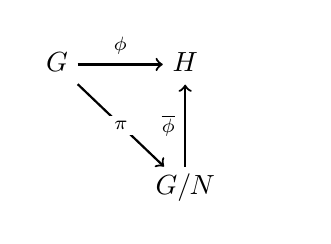
\begin{tikzpicture}[description/.style={fill=white,inner sep=2pt}]
\matrix (m) [matrix of math nodes, row sep=3em,
column sep=2.5em, text height=1.5ex, text depth=0.25ex]
{ G & H \\
& G/N & \\ };
\path[->,font=\scriptsize]
(m-1-1) edge[thick] node[auto] {$ \phi $} (m-1-2)
edge[thick] node[description] {$ \pi $} (m-2-2)
(m-2-2)[thick] edge node[auto] {$ \overline{\phi} $} (m-1-2);
\end{tikzpicture}
\end{wrapfigure}

It is convenient here to introduce the concept of a commutative diagram. A commutative diagram is a directed graph where vertices are sets and edges are functions between the sets it connects, with the following property. If there are two paths $S \xrightarrow{f_1} A_1 \xrightarrow{f_2} \dots \xrightarrow{f_{n-1}} A_n \xrightarrow{f_n} E$, and $S \xrightarrow{g_1} B_1 \xrightarrow{g_2} \dots \xrightarrow{f_{m-1}} B_m \xrightarrow{g_m} E$ from $S$ to $E$, then $f_n \circ \dots \circ f_1 = g_m \circ \dots \circ f_1$. An example diagram is to the left, representing the functions in the first isomorphism theorem.

Let $\langle g \rangle$ be a cyclic group. Define a surjective homomorphism from $\mathbf{Z}^+$ $r \mapsto g^r$. If $\langle g \rangle$ is order $n$, $n\mathbf{Z}^+$ is the kernel of the map. Then $\langle g \rangle \cong \mathbb{Z}^+/n\mathbb{Z}^+$. If $\langle g \rangle$ is infinite, the kernel of the map is $\{ 0 \}$, and $\mathbb{Z}^+/0\mathbb{Z}^+ \cong \mathbb{Z}^+$, so $\langle g \rangle \cong \mathbb{Z}^+$.

Another useful theorem is the second isomorphism theorem. Let $G$ be a group, and $N$ and $H$ subgroups such that $N$ is normal in $G$. The $NH$ is a subgroup of $G$, and $N \cap H$ is normal in $G$. The assignment map $h(N \cap H) \mapsto hN$ is an isomorphism, and so $H/N \cap H$ is isomorphic to $NH/H$:
\begin{proof}
    First we prove $NH$ is a subgroup. If $n_1h_1$ and $n_2h_2$ are in $NH$, then $n_1h_1(n_2h_2)^{-1}$ is in $NH$ by the following calculation:

    \begin{align*}
    n_1h_1(n_2h_2)^{-1} &= n_1h_2h_2^{-1}n_2^{-1}\\
    &= n_1(h_1h_2^{-1}n_2^{-1}(h_1h_2^{-1})^{-1})h_1h_2^{-1}
    \end{align*}

    The equation above is in $NH$ as $N$ is normal. The map $h \mapsto hN$ is a surjective homomorphism from $H$ to $NH/N$, and the kernel is $N \cap H$, so $H/N \cap H \cong NH/N$.
\end{proof}

The final isomorphism is the third isomorphism theorem. If $M$ and $N$ are normal subgroups of a group $G$, where $N$ is also a normal subgroup of $M$. Then $M/N$ is a subgroup of $G/N$, and $(G/N)/(M/N) \cong G/M$:
\begin{proof}
    The assignment $gN \mapsto gM$ is a surjective homomorphism, well defined as $N$ is a subgroup of $M$. The kernel of this map are all cosets of $M$ that are cosets of $M/N$. By the first isomorphism theorem, $(G/N)/(M/N) \cong G/M$.
\end{proof}

\section{Product Groups}

Let $I$ be an index set, and $\{ G_i \}_{i \in I}$ a family of groups. Then the direct product of $\{ G_i \}$, denoted $\varprod_{i \in I} G_i$, is a group with operation $\varprod_{i \in I} g_i \circ \varprod_{i \in I} h_i = \varprod_{i \in I} g_ih_i$. The group is called the product group.

Let $r$ and $s$ be two relatively prime integers. Suppose $G$ is a cyclic group of order $rs$. Then $G$ is isomorphic to the direct product of cyclic groups $R$ and $S$, where $R$ is order $r$ and $S$ is order $s$.
\begin{proof}
    $R \times S$ is a cyclic group generated by $(x,y)$, where $x^r = e$, and $y^s = e$. This follows as $(x,y)^{rs} = (x^{rs},y^{rs}) = (e,e)$. If $(x,y)^m = (x^m,y^m) = (e,e)$, $r|m$ and $s|m$, so $rs|m$.
\end{proof}

Let $H$ and $K$ be normal subgroups of a group $G$, such that $H \cap K = \{ e \}$, and $HK = G$. Then $H \times K \cong G$:
\begin{proof}
    Define a map $(h,k) \mapsto hk$. The map is bijective, as $HK = G$, and if $hk = e$, $h = k^{-1}$, so $k^{-1} \in H$, so $k = h = e$. $hkh^{-1} \in K$, as $K$ is normal, but it is also in $N$ as $N$ is normal, hence $hkh^{-1}k^{-1} = e$, so $hk = kh$, and thus the map is a homomorphism as $h_1k_1h_2k_2 = h_1h_2k_1k_2$.
\end{proof}

\chapter{Group Actions}

Automorphisms are symmetries form groups over a set. These are specific notions of a more general structure, a group action. A group action or operation on a set $G$ and set $X$ is a homomorphism from $G$ to $S_X$. As each $g \in G$ has an associated permutation, we write for $s \in S$, $gs$ for the permutation associated with $g$ action on $s$. We call $S$ a $G$-set. It is simple to show $g(hx) = (gh)x$ and $ex = x$.

Given a group $G$, and a $G$-set $S$, for $s \in S$, let the orbit of $s$ be $Gs$, the set of all $gs$ for $g \in G$. The relation $x \sim y$ if $Gx = Gy$ is an equivalence relation and partitions the set into orbits of $S$. Note that this means the group acts independently on each of a $G$-set's orbits. A $G$-set is transitive if it has just one orbit. An action is faithful if it is injective. A map $\phi$ froma  $G$-set $X$ to a $G$-set $Y$ is a $G$-morphism if $\phi(gx) = g\alpha(x)$ for all $g \in G$ and $x \in X$. $\phi$ is an isomorphism if it is bijective.

An element $x$ in a $G$-set $X$ is a fixed point if $gx = x$ for every $g \in G$. The set of all fixed points is denoted $X^G$. Given any $x \in X$, $G_x = \{ g \in G | gx = x \}$ is a subgroup called the isotropy subgroup of $x$ in $G$.

As an example, let $G$ act on itself by conjugation $g(h) = ghg^{-1}$. The isotopy subgroups are called centralizers $C_G(h) = \{ g \in G | gh = hg \}$. A fixed point is a center, and the set of all centers is denoted $Z(G)$.

Consider conjugation from $G$ on its subgroups. Then the isotropy group of a subgroup $H$ is the normalizer $N_G(H)$, which is the set $\{ g \in G | gHg^{-1} = H \}$. The fixed points are the normal subgroups.

Consider the group $SL_n(\mathbf{R})$ acting on the upper half of the complex plane $H = \{ z \in \mathbf{C} | \im(z) > 0 \}$ by the mobius transform below:

\[\begin{pmatrix} a & b \\ c & d \end{pmatrix} z = \frac{az + b}{cz + d}\]

The isotropy subgroup of $i$ is the special orthogonal group $SO(2)$, the set of matrices with orthonormal columns. The mobius transform is transitive. A meromorphic function on $H$ invariant under $SO(2)$ is called a modular function, and is essential to the study of number theory, string theory, and the study of monstrous moonshine.

\end{document}